\documentclass[submit]{harvardml}

% Put in your full name and email address.
\name{Mingu K., Catherine W., Hugo Y.}

% You don't need to change these.
\course{CS181-S16}
\assignment{Practical \#2}
\duedate{4:59pm Mar 4, 2016}

\usepackage[OT1]{fontenc}
\usepackage[colorlinks,citecolor=blue,urlcolor=blue]{hyperref}
\usepackage[pdftex]{graphicx}
\usepackage{subfig}
\usepackage{fullpage}
\usepackage{palatino}
\usepackage{mathpazo}
\usepackage{amsmath}
\usepackage{amssymb}
\usepackage{indentfirst}
\usepackage{color}
\usepackage{todonotes}
\usepackage{listings}
\usepackage{float}
\usepackage{common}
\usepackage{bm}

\usepackage[mmddyyyy,hhmmss]{datetime}

\definecolor{verbgray}{gray}{0.9}

\lstnewenvironment{csv}{%
  \lstset{backgroundcolor=\color{verbgray},
  frame=single,
  framerule=0pt,
  basicstyle=\ttfamily,
  columns=fullflexible}}{}


\begin{document}
\begin{center}
{\Large Practical 2: Classifying Malicious Software}\\
\end{center}
\vspace{4mm}
\subsection*{Technical Approach}
\iffalse
How did you tackle the problem? Credit will be given for
• Diving deeply into a method (rather than just trying off-the-shelf tools with default
settings) and making tuning and configuration decisions using thoughtful
experimentation.
• Exploring several methods, perhaps going beyond those we discussed in class.
In either/both routes, thoughtfully iterating on approaches is key. If you used existing
packages or referred to papers/blogs for ideas, you should cite these in your
report.
\fi

Our final submission used random forest (RF) classification to train data on features that were specifically chosen to be virus-type specific. From the beginning, we knew that feature engineering would be an important part of fitting the data well. Thus, we found our features by using grepWin (http://stefanstools.sourceforge.net/grepWin.html), a grep client that allows us to search strings in each of the xml files in our directory. It allowed us to search different words or phrases to see if a disproportionate amount of matches were found in xml files of a particular virus type. By inspection, we could see a number of suspicious phrases, such as ``00 00 00 00 00 00 00 00" and ``CREATE\_ SUSPENDED", and try looking at the frequency of matches in each xml file. For example, the latter phrase appeared almost exclusively for Swizzor xmls, so we knew that the number of matches for this phrase would be an important feature for our classification.\\

	For our best result, we used 14 features for our classification. The majority of our attempts for optimization came from generating new features and testing them to see the effect on the error. After iterating like this for several different sets of features, we expanded to test other types of classification methods, including logistic and radial basis function (RBF) network classifiers. However, we soon figured out that the random forest classifier was the best method to use, which was our first Kaggle submission.\\



\subsection*{Results}
\iffalse
Did you create and submit a set of predictions? Did your methods give reasonable
performance? Credit will be given for quantitatively reporting (with clearly
labeled and captioned figures and/or tables) on the performance of the methods
you tried compared to your baselines. You must have at least one plot or table that
details the performances of different methods tried. You will not be graded in proportion
to your ranking; we’ll be using the ranking to help calibrate how difficult the
task was and to award bonus points to those who go above and beyond. However,
you must at least clear any sample baseline scores shown on the Kaggle leaderboard
to earn full points.
\fi

\begin{table}[H]
\centering
\caption{Classification Accuracy for successive trials - displays the accuracy for the different trials that we performed, as well as the change that were made between each trial to better understand the effectiveness of various changes}
\label{my-label}
\begin{tabular}{|l|l|l|l|}
\hline
\textbf{Trial \#} & \textbf{Total \# of Features} & \textbf{Changes}    & \textbf{Kaggle Accuracy} \\ \hline
Baseline          & -                             & -                   & 0.39000                  \\ \hline
1                 & 14                            & RF Classifier       & 0.71263                  \\ \hline
2                 & 14                            & Logistic Classifier & 0.64105                  \\ \hline
3                 & 14                            & RBF Classifier      & 0.59105                  \\ \hline
4                 & 34                            & RF- 34 features     & 0.70316                  \\ \hline
5                 & 30                            & RF- 30 features     & 0.70105                  \\ \hline
\end{tabular}
\end{table}

\begin{figure}[H]
\centering
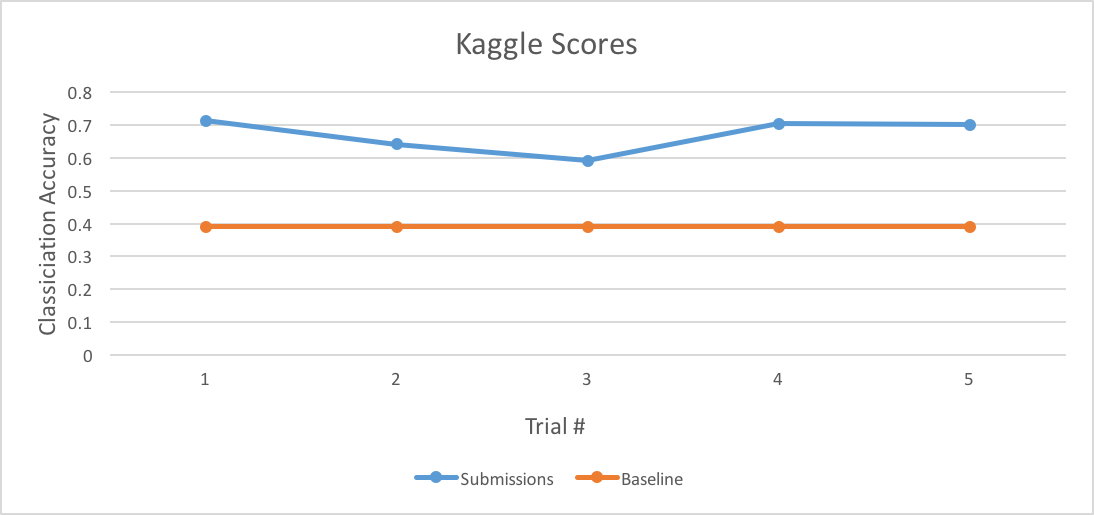
\includegraphics[width=1.0 \textwidth]{Kaggle_graph.png}
\caption*{Graph 2: Graph of Accuracy over time - a graph of our official Kaggle Classification Accuracy scores with successive trials. All of our results were above the baseline measure, but we tried improving our score by using different classifiers and features. However, our first submission was our best submission, probably due to overfitting.}
\end{figure}

\subsection*{Discussion}
\iffalse
Do you explain not just what you did, but your thought process for
your approach? Credit will be given for
• Explaining the your reasoning for why you seqentially chose to try the approaches
you did (i.e. what was it about your initial approach that made you
try the next change?).
• Explaining the results. Did the adaptations you tried improve the results? Why
or why not? Did you do additional tests to determine if your reasoning was
correct?
\fi

\noindent \textbf{The first trial} \\

We began by identifying phrases that were disproportionately found in one or a few virus types to use as features. It was clear from the beginning that string parsing would be a key component to the practical, and we needed an easy way to check the frequencies of words in the xml files that could be used to distinguish all the xml files from each other. Furthermore, as a group we felt that feature extraction would be more important to accurate classification than fancy methods, and so we wanted to make sure that we would get the most representative features possible. Therefore, we came across grepWin, which would allow us to do just this. By using grepWin, it was easy to compare matches vs virus type, and we kept a spreadsheet of features that we wanted to use in our classification. We searched for these features in the metadata of elements inside the xml files, and we noted the viruses that each phrase was associated with (FeatureExtractionInformation.xlsx). Using this process, we were able to initially find 14 potentially useful features for our classification that we wanted to start with. \\

After finding these features, we exported a table to Excel with the number of matches we found for each phrase in the training data from each xml file (Features.xlsx). This would be the data table that we used for classification purposes. We also generated this data table for the test data (TestFeatures.xlsx). We could then simply import the table as data and wrote a script that would use RF classification to generate our output file for Kaggle submission. After submitting, we got an initial score of 0.71263, which was exciting to see because we outperformed the baseline measure for our first submission. \\

\noindent \textbf{Trying different classification methods} \\

Next, we tried using different classification methods to see if we could use a different method on the same features to improve our score. However, after implementing them in our script, we soon realized that RF classification performed better than other methods. We tried using both logistic and RBF classification, both of which did better than the baseline but not as well as RF classification (as shown in Table 1 in the Results section). Thus, we decided to stick with RF classification. \\

\noindent \textbf{Trying different features} \\

Finally, we tried to improve our score by using different features for our analysis. We figured that if RF classifiers were underfitting the data, then introducing more relevant features could improve our score. However, if adding features made our score worse, we would suppose that the added features were overfitting the training data. Thus, we used the same method outlined in the first trial section, and found 20 more features for a total of 34 features in our data, and added all this information in the virus/phrase association information spreadsheet mentioned previously (FeatureExtractionInformation.xlsx). We then exported this data as a table as well for classification analysis for our test data (TestFeatures.xlsx). After RF classification with these features, however we discovered that we performed worse, indicating that we were overfitting our training data and not generalizing to our test set well. Thus, we removed the 4 features that we felt were least meaningful (``Travel Insurance.url'', ``Dokumente'', ``URLOpenBlockingStream'', ``WH\_ MOUSE''), and tried running our script again. We still did not improve our initial set of 14 features, indicating that our first trial did the best job with generalizing to the test set. \\

If we had more time, we could have tried using other feature extraction methods. However, all of our methods performed better than the baseline, indicating good performance from our feature extraction and our classification methods used.



\end{document}